\chapter{Архивация данных} \label{chapt8}%
\textbf{Мета роботи:~}%
Выполнить исследование алгоритмов архивации данных. Использовать алгоритм
Хаффмана и Лемпеля-Зива для архивации. Восстановить данные после
\section{Теоретические ведомости} \label{sect8_a}
% Лабораторная 9
\paragraph{Архивация данных}

\textbf{Архивация (сжатие данных)} --- есть процесс представления информации
в ином виде (перекодирования) с потенциальным уменьшением объёма, требуемого
для её хранения. Существует множество классов различных алгоритмов сжатия
данных, каждый из которых ориентирован на свою область применения.
\href{http://studopedia.ru/9_131056_simmetrichnie-kriptosistemi.html}{Источник}

Основоположником науки о сжатии информации принято считать \emph{Клода
Шеннона}. Его теорема об оптимальном кодировании показывает, к чему нужно
стремиться при кодировании информации и насколько та или иная информация при
этом сожмется. Кроме того, им были проведены опыты по эмпирической оценке
избыточности английского текста. Шенон предлагал людям угадывать следующую
букву и оценивал вероятность правильного угадывания. На основе ряда опытов он
пришел к выводу, что количество информации в английском тексте колеблется в
пределах $0,6 – 1,3$ бита на символ. Несмотря на то, что результаты
исследований Шеннона были по-настоящему востребованы лишь десятилетия спустя,
трудно переоценить их значение.

\textbf{Сжатие данных} --- это процесс, обеспечивающий уменьшение объёма
данных путём сокращения их избыточности. Сжатие данных связано с компактным
расположением порций данных стандартного размера. Сжатие данных можно
разделить на два основных типа:


\textbf{Сжатие без потерь} (полностью обратимое) --- это метод сжатия данных,
при котором ранее закодированная порция данных восстанавливается после их
распаковки полностью без внесения изменений. Для каждого типа данных, как
правило, существуют свои оптимальные алгоритмы сжатия без потерь.

\textbf{Сжатие с потерями} --- это метод сжатия данных, при котором для
обеспечения максимальной степени сжатия исходного массива данных часть
содержащихся в нём данных отбрасывается. Для текстовых, числовых и табличных
данных использование программ, реализующих подобные методы сжатия, является
неприемлемыми. В основном такие алгоритмы применяются для сжатия аудио и
видеоданных, статических изображений.

\paragraph{Алгоритмы архивации данных}

\textbf{Алгоритм сжатия данных} --- это алгоритм, который устраняет
избыточность записи данных.

\textbf{Отношение сжатия} --- одна из наиболее часто используемых величин для
обозначения эффективности метода сжатия.
\begin{equation}\label{Otnosh_Schatia}
 \text{Отношение сжатия} = \frac{\text{размер
выходного потока}}{\text{размер входного потока}}
\end{equation}
Значение 0,6 означает, что данные занимают 60\% от первоначального объема.
Значения больше 1 означают, что выходной поток больше входного (отрицательное
сжатие, или расширение).

\textbf{Коэффициент сжатия} --- величина, обратная отношению сжатия.

\begin{equation}\label{Otnosh_Schatia}
 \text{Коэффициент сжатия} = \frac{\text{размер входного потока}}{\text{размер
выходного потока}}
\end{equation}
Значения больше 1 обозначают сжатие, а значения меньше 1 расширение.

\textbf{Средняя длина кодового слова} -- это величина, которая вычисляется
как взвешенная вероятностями сумма длин всех кодовых слов.

\begin{equation}
L_{cp}=p_1 \cdot L_1 + p_2 \cdot L_2 +\ldots + p_n \cdot L_n ,
\end{equation}
где $p_n$ -- вероятности кодовых слов,
    $L_1,L_2,L_3$ -- длины кодовых слов.

\textbf{Статистические методы} --- методы сжатия, присваивающие коды
переменной длины символам входного потока, причем более короткие коды
присваиваются символам или группам символам, имеющим большую вероятность
появления во входном потоке. Лучшие статистические методы применяют
кодирование Хаффмана.

\textbf{Словарное сжатие} --- это методы сжатия, хранящие фрагменты данных в
"словаре" (некоторая структура данных). Если строка новых данных, поступающих
на вход, идентична какому-либо фрагменту, уже находящемуся в словаре, в
выходной поток помещается указатель на этот фрагмент. Лучшие словарные методы
применяют метод Зива-Лемпела.

Рассмотрим несколько известных алгоритмов сжатия данных более подробно.

\subparagraph{Алгоритм Хаффмана}

В основе алгоритма Хаффмана лежит идея кодирования битовыми группами. Сначала
проводится частотный анализ входной последовательности данных, то есть
устанавливается частота вхождения каждого символа, встречащегося в ней. После
этого, символы сортируются по уменьшению частоты вхождения.

Основная идея состоит в следующем: чем чаще встречается символ, тем меньшим
количеством бит он кодируется. Результат кодирования заносится в словарь,
необходимый для декодирования. Рассмотрим простой пример, иллюстрирующий
работу алгоритма Хаффмана.

Пусть задан текст <<beep boop beer!>>, рассмотрим таблицу с частотами всех
символов:

\begin{table} [!htbp]% Пример записи таблицы с номером, но без отображаемого наименования
  \centering
  \parbox{8cm}%
  {% чтобы лучше смотрелось, подбирается самостоятельно
    \caption{Частота символов}%
    \label{tabl:tab8x1}%
    \begin{SingleSpace}
    \begin{tabular}{lccccccc}
    \hline
    \multicolumn{1}{|l|}{\textbf{Символ}}                          & \multicolumn{1}{c|}{'b'}                       & \multicolumn{1}{c|}{'e'}                       & \multicolumn{1}{c|}{'p'}                       & \multicolumn{1}{c|}{' '}                       & \multicolumn{1}{c|}{'o'}                       & \multicolumn{1}{c|}{'r'}                       & \multicolumn{1}{c|}{'!'}                       \\ \hline
    \rowcolor[HTML]{EFEFEF}
    \multicolumn{1}{|l|}{\cellcolor[HTML]{EFEFEF}\textbf{Частота}} & \multicolumn{1}{c|}{\cellcolor[HTML]{EFEFEF}3} & \multicolumn{1}{c|}{\cellcolor[HTML]{EFEFEF}4} & \multicolumn{1}{c|}{\cellcolor[HTML]{EFEFEF}2} & \multicolumn{1}{c|}{\cellcolor[HTML]{EFEFEF}2} & \multicolumn{1}{c|}{\cellcolor[HTML]{EFEFEF}2} & \multicolumn{1}{c|}{\cellcolor[HTML]{EFEFEF}1} & \multicolumn{1}{c|}{\cellcolor[HTML]{EFEFEF}1} \\ \hline
    \\
    \multicolumn{8}{c}{По частоте использования}                                                                                                                                                                                                                                                                                                                                                                             \\ \hline
    \multicolumn{1}{|l|}{\textbf{Символ}}                          & \multicolumn{1}{c|}{'r'}                       & \multicolumn{1}{c|}{'!'}                       & \multicolumn{1}{c|}{'p'}                       & \multicolumn{1}{c|}{'o'}                       & \multicolumn{1}{c|}{' '}                       & \multicolumn{1}{c|}{'b'}                       & \multicolumn{1}{c|}{'e'}                       \\ \hline
    \end{tabular}
    \end{SingleSpace}
    }
\end{table}

После этого создадим элементы бинарного дерева для каждого символа и
представим их как очередь с приоритетом, в качестве которого будем
использовать частоту.

Возьмём первые два элемента из очереди и создадим третий, который будет их
родителем. Этот новый элемент поместим в очередь с приоритетом, равным сумме
приоритетов двух его потомков. Иначе говоря, равным сумме их частот.

%2
\begin{figure}[!htbp]
  \centering
  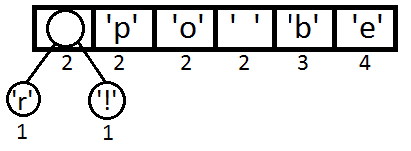
\includegraphics[width=\linewidth/3]{img8x2}
  \caption{2}\label{img:8x2}
\end{figure}
Далее будем повторять шаги, аналогичные предыдущему:

%3-6
\begin{figure}[!htbp]
  \centering
  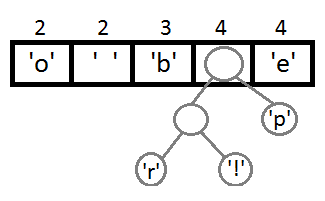
\includegraphics[width=\linewidth/3]{img8x3}
  \label{img:8x3}

  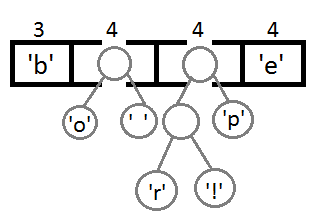
\includegraphics[width=\linewidth/3]{img8x4}
  \label{img:8x4}

  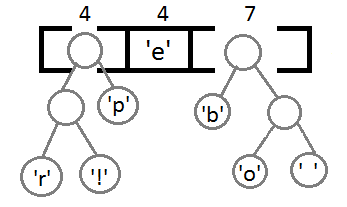
\includegraphics[width=\linewidth/3]{img8x5}
  \label{img:8x5}

  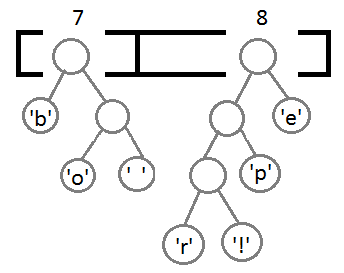
\includegraphics[width=\linewidth/3]{img8x6}
  \caption{Построение дерева}\label{img:8x6}
\end{figure}

Теперь, после объединения последних двух элементов с помощью их нового
родителя, мы получим итоговое бинарное дерево:
%7
\begin{figure}[!htbp]
  \centering
  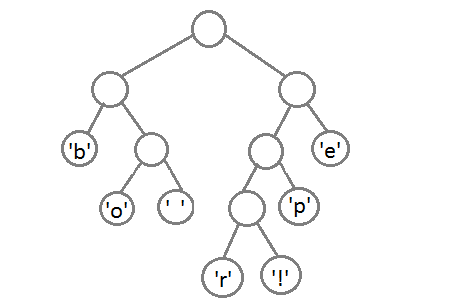
\includegraphics[scale=0.6]{img8x7}
  \caption{7}\label{img:8x7}
\end{figure}
Осталось присвоить каждому символу его код. Для этого запустим обход в
глубину и каждый раз, рассматривая правое поддерево, будем записывать в код
1, а рассматривая левое поддерево — 0.

\begin{figure}[!htbp]
  \centering
  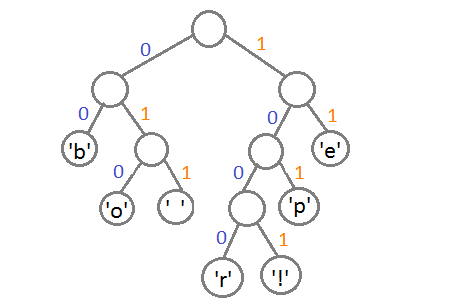
\includegraphics[scale=0.6]{img8x8}
  \caption{8}\label{img:8x8}
\end{figure}
%8

В результате соответствие символов кодовым значениям получится следующим:
\begin{table} [!htbp]% Пример записи таблицы с номером, но без отображаемого наименования
  \centering
  \parbox{12cm}%
  {% чтобы лучше смотрелось, подбирается самостоятельно
    \caption{Кодовые значения символов}%
    \label{tabl:tab8x2}%
    \begin{SingleSpace}
    \begin{tabular}{|l|c|c|c|c|c|c|c|}
    \hline
    \textbf{Сивол}            & ‘b’ & ‘e’ & ‘p’ & ‘ ‘ & ‘o’ & ‘r’  & ‘!’  \\ \hline
    \rowcolor[HTML]{EFEFEF}
    \textbf{Кодовое значение} & 00  & 11  & 101 & 011 & 010 & 1000 & 1001 \\ \hline
    \end{tabular}
    \end{SingleSpace}
    }
\end{table}

Декодирование битов происходит следующим образом: нужно обходить дерево,
отбрасывая левое поддерево, если встретилась единица и правое, если
встретился 0. Продолжать обход нужно до тех пор, пока не встретим лист, т.е.
искомое значение закодированного символа. Например, закодированной строке
<<101 11 101 11>> и нашему дереву декодирования соответствует строка <<pepe>>

\noindent \textbf{Входная строка: }<<beep boop beer!>>

\noindent \textbf{Входная строка в двоичном виде:} 0110 0010 0110 0101 0110
0101 0111 0000 0010 0000 0110 0010 0110 1111 0110 1111 0111 0000 0010 0000
0110 0010 0110 0101 0110 0101 0111 0010 0010 0001

\noindent \textbf{Закодированная строка:} 0011 1110 1011 0001 0010 1010 1100
1111 1000 1001

Разница между ASCII-кодировкой строки и её же видом в коде Хаффмана очевидна.

Алгоритм Хаффмана универсальный, его можно применять для сжатия данных любых
типов, но он малоэффективен для файлов маленьких размеров (за счет
необходимости сохранения словаря). В настоящее время данный метод практически
не применяется в чистом виде, обычно используется как один из этапов сжатия в
более сложных схемах. Это единственный алгоритм, который не увеличивает
размер исходных данных в худшем случае (если не считать необходимости хранить
таблицу перекодировки вместе с файлом).

\subparagraph{Алгоритм Лемпеля-Зива}

Процесс сжатия выглядит следующим образом. Последовательно считываются
символы входного потока и происходит проверка, существует ли в созданной
таблице строк такая строка. Если такая строка существует, считывается
следующий символ, а если строка не существует, в поток заносится код для
предыдущей найденной строки, строка заносится в таблицу, а поиск начинается
снова. Например, если сжимают байтовые данные (текст), то строк в таблице
окажется 256 (от <<0>> до <<255>>). Если используется 10-битный код, то под
коды для строк остаются значения в диапазоне от 256 до 1023. Новые строки
формируют таблицу последовательно, т. е. можно считать индекс строки ее
кодом. Алгоритму декодирования на входе требуется только закодированный
текст, поскольку он может воссоздать соответствующую таблицу преобразования
непосредственно по закодированному тексту. Алгоритм генерирует однозначно
декодируемый код за счет того, что каждый раз, когда генерируется новый код,
новая строка добавляется в таблицу строк. LZW постоянно проверяет, является
ли строка уже известной, и, если так, выводит существующий код без генерации
нового. Таким образом, каждая строка будет храниться в единственном
экземпляре и иметь свой уникальный номер. Следовательно, при дешифровании при
получении нового кода генерируется новая строка, а при получении уже
известного, строка ивлекается из словаря.
\href{https://habrahabr.ru/post/132683/}{[ссылка]}

\noindent\textbf{Кодирование}

Пусть мы сжимаем последовательность <<abacabadabacabae>>.
\begin{enumerate}
\item Тогда, согласно изложенному выше алгоритму, мы добавим к изначально
    пустой строке <<a>> и проверим, есть ли строка <<a>> в таблице. Поскольку мы
    при инициализации занесли в таблицу все строки из одного символа, то
    строка <<a>> есть в таблице.
\item Далее мы читаем следующий символ «b>> из входного потока и проверяем,
    есть ли строка <<ab>> в таблице. Такой строки в таблице пока нет.
\item Добавляем в таблицу <5> <<ab>>. В поток: <0>;
\item <<ba>> — нет. В таблицу: <6> <<ba>>. В поток: <1>;
\item <<ac>> — нет. В таблицу: <7> <<ac>>. В поток: <0>;
\item <<ca>> — нет. В таблицу: <8> <<ca>>. В поток: <2>;
\item <<ab>> — есть в таблице; <<aba>> — нет. В таблицу: <9> <<aba>>. В
    поток: <5>;
\item <<ad>> — нет. В таблицу: <10> <<ad>>. В поток: <0>;
\item <<da>> — нет. В таблицу: <11> <<da>>. В поток: <3>;
\item <<aba>> — есть в таблице; <<abac>> — нет. В таблицу: <12> <<abac>>. В
    поток: <9>;
\item <<ca>> — есть в таблице; <<cab>> — нет. В таблицу: <13> <<cab>>. В
    поток: <8>;
\item <<ba>> — есть в таблице; <<bae>> — нет. В таблицу: <14> <<bae>>. В
    поток: <6>;
\item И, наконец последняя строка <<e>>, за ней идет конец сообщения,
    поэтому мы просто выводим в поток <4>.
\end{enumerate}
\begin{figure}[!htbp]
  \centering
  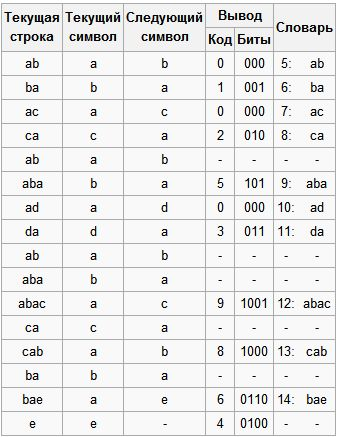
\includegraphics[scale=0.8]{img8x9}
  \caption{9}\label{img:8x9}
\end{figure}
Мы получаем закодированное сообщение <<0 1 0 2 5 0 3 9 8 6 4>>, что на
11-бит короче.\\
\vspace{1cm}
\\
\noindent\textbf{Декодирование}

Особенность LZW заключается в том, что для декомпрессии нам не надо сохранять
таблицу строк в файл для распаковки. Алгоритм построен таким образом, что мы
в состоянии восстановить таблицу строк, пользуясь только потоком кодов.
Теперь представим, что мы получили закодированное сообщение, приведённое
выше, и нам нужно его декодировать. Прежде всего, нам нужно знать начальный
словарь, а последующие записи словаря мы можем реконструировать уже на ходу,
поскольку они являются просто конкатенацией предыдущих записей.
\begin{figure}[!htbp]
  \centering
  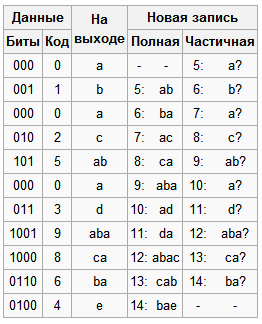
\includegraphics[scale=0.9]{img8x10}
  \caption{10}\label{img:8x10}
\end{figure}

\noindent\textbf{Достоинства и недостатки}
\begin{description}
  \item[+] Не требует вычисления вероятностей встречаемости символов или
      кодов.
  \item[+] Для декомпрессии не надо сохранять таблицу строк в файл для
      распаковки. Алгоритм построен таким образом, что мы в состоянии
      восстановить таблицу строк, пользуясь только потоком кодов.
  \item[+] Данный тип компрессии не вносит искажений в исходный графический
      файл, и подходит для сжатия растровых данных любого типа.
  \item[-]Алгоритм не проводит анализ входных данных поэтому не оптимален.
\end{description}

\section{Задания}\label{sect8_b}
%https://studfiles.net/preview/5855938/
\begin{enumerate}
  \item Взять данные соответственно варианту из \todo{табл.}
  \item Удалить лишнюю информацию методом Хаффмана.
  \item Провести операцию методом Лемпеля-Зива.
  \item Сравнить результаты проведённых операций.
  \item Описать актуальность архивации.
  \item Сделать выводы по применению методов сжатия в различных
      криптосистемах.
\end{enumerate}
\section{Пример выполнения работы}\label{sect8_c}
%
\section{Варианты}\label{sect8_d}
%
\section{Вопросы для контроля}\label{sect8_e}
%
\begin{enumerate}
  \item Что такое архивация данных?
  \item Цель архивации?
  \item Какие Вы знаете методы архивации?
  \item Опишите принцип дерева Хаффмана.
  \item Опишите алгоритм LZ77 или его аналог.
  \item Сферы применения заданных алгоритмов.
  \item Как выбрать алгоритм, если данные заранее известны?
\end{enumerate}
